\documentclass{article}

% Document packages
\usepackage[utf8]{inputenc} % Input encoding
\usepackage[T1]{fontenc} % Font encoding
\usepackage[english]{babel} % Language
\usepackage{listings} % For verbatim environment
\usepackage{tikz}

% Page layout
\usepackage{geometry} % Adjust margins
\geometry{a4paper, margin=1in} % Set margins

% Title information
\title{Database Management System \\ CSE 2221}
\author{Noortaz Rezoana}
\date{April 2024}

\begin{document}

\maketitle

% Your content goes here
\newpage
\section*{Chapter 1: Introduction}

\subsection*{Data Definition Language (DDL)}

Specification notation is a formal way to define the structure of a database schema. In the example provided, we use SQL (Structured Query Language) to specify the creation of a table named "instructor" with four columns: ID, name, dept\_name, and salary. Each column has a specified data type and length.

\begin{lstlisting}[language=SQL]
create table instructor (
    ID                char(5),
    name           varchar(20),
    dept_name  varchar(20),
    salary           numeric(8,2)
)
\end{lstlisting}

When we execute this SQL statement, a Data Definition Language (DDL) compiler generates a set of table templates stored in a data dictionary. This data dictionary serves as a repository for metadata, which is essentially data about the data. 

The data dictionary includes crucial information such as:

\begin{itemize}
    \item \textbf{Database Schema}: The overall structure of the database, including tables, columns, and their data types.
    \item \textbf{Integrity Constraints}: Rules that enforce the validity and consistency of data, such as ensuring that certain fields cannot be left blank or that values in one table match values in another.
    \item \textbf{Primary Key}: A unique identifier for each record in a table. In our example, the "ID" column serves as the primary key, ensuring that each instructor has a unique identifier.
    \item \textbf{Authorization}: Specifies who can access what data within the database. This includes permissions for reading, writing, updating, and deleting data, ensuring data security and privacy.
\end{itemize}

By utilizing specification notation and maintaining a data dictionary, database administrators can effectively manage the structure, integrity, and security of their databases.

\subsection*{Data Manipulation Language (DML)}

Data Manipulation Language (DML) is a language used for accessing and updating the data organized by the appropriate data model. DML is also commonly referred to as a query language.

There are two primary types of Data Manipulation Language:

\begin{enumerate}
    \item \textbf{Procedural DML}: Procedural DML requires a user to specify what data are needed and how to get those data. In other words, it involves step-by-step instructions on how to manipulate the data.
    
    \item \textbf{Declarative DML}: Declarative DML, on the other hand, requires a user to specify what data are needed without specifying how to get those data. Instead of giving detailed instructions, declarative DML focuses on stating the desired outcome. Declarative DMLs are usually easier to learn and use than procedural DMLs. They are also referred to as non-procedural DMLs.
\end{enumerate}

$\theta$ The portion of a DML that involves information retrieval is called a query language. Query languages allow users to retrieve specific data from a database based on defined criteria.

$\theta$ Procedural DMLs provide a detailed approach to data manipulation, requiring users to specify each step of the process. While this can offer more control, it often requires a deeper understanding of the underlying mechanisms.

$\theta$ In contrast, declarative DMLs abstract away the implementation details, allowing users to focus on the desired outcome rather than the specific steps needed to achieve it. This makes them more intuitive and user-friendly, particularly for those without extensive programming experience.

$\theta$ By understanding the distinctions between procedural and declarative DMLs, database users can choose the most appropriate approach based on their specific needs and expertise.

\newpage




\subsection*{SQL Query Language}

SQL (Structured Query Language) is a nonprocedural query language commonly used for managing and manipulating relational databases. Unlike procedural languages, SQL focuses on specifying what data is needed rather than how to retrieve it.

A SQL query takes as input one or more tables and always returns a single table as output. For example, to find all instructors in the Computer Science department, we can use the following SQL query:

\begin{verbatim}
select name
from instructor
where dept_name = 'Comp. Sci.'
\end{verbatim}

SQL is not a Turing machine equivalent language, meaning it does not have the computational power to perform arbitrary computations like a Turing machine. Instead, SQL is designed specifically for querying and manipulating relational databases.

To perform complex computations, SQL is often embedded within higher-level programming languages. Application programs typically access databases through one of two methods:

\begin{enumerate}
    \item \textbf{Language Extensions}: Some programming languages provide extensions to embed SQL directly within the code. This allows seamless integration of database operations with application logic.
    
    \item \textbf{Application Program Interface (API)}: APIs such as ODBC (Open Database Connectivity) and JDBC (Java Database Connectivity) provide a standardized way for applications to communicate with databases. These APIs allow SQL queries to be sent to a database and retrieve results programmatically.
\end{enumerate}

By leveraging SQL and appropriate interfaces, developers can efficiently interact with databases and incorporate data manipulation capabilities into their applications.



\subsection*{Database Design}

Database design is the process of designing the general structure of a database to efficiently store and manage data. It involves making decisions about the logical and physical organization of the database.

\subsubsection*{Logical Design}

Logical design focuses on deciding the database schema, which involves determining the structure of the database at a conceptual level. This stage of database design requires finding a "good" collection of relation schemas that accurately represent the data and support the required functionality.

During logical design, several key decisions are made:

\begin{itemize}
    \item \textbf{Business Decision}: What attributes should be recorded in the database? This involves understanding the requirements of the business or organization and identifying the essential data elements to be stored.
    
    \item \textbf{Computer Science Decision}: What relation schemas should be created, and how should the attributes be distributed among them? This decision involves translating business requirements into database structures, determining the entities, attributes, and relationships that need to be represented.
\end{itemize}

\subsubsection*{Physical Design}

Physical design focuses on deciding the physical layout of the database, including storage structures, indexing, and optimization techniques. This stage aims to optimize the performance and efficiency of database operations by organizing data in a way that minimizes storage requirements and maximizes access speed.

During physical design, considerations include:

\begin{itemize}
    \item Storage organization, such as file organization and indexing methods.
    \item Data compression and encryption techniques for security and resource optimization.
    \item Optimization of query performance through indexing, partitioning, and caching strategies.
\end{itemize}

By carefully designing the logical and physical structure of the database, database designers can ensure that the database meets the requirements of the organization while optimizing performance and resource utilization.



\subsection*{Query Processor}

The query processor is a crucial component of a database management system responsible for interpreting and executing queries. It consists of several key components:

\begin{itemize}
    \item \textbf{DDL Interpreter}: The Data Definition Language (DDL) interpreter interprets DDL statements, such as creating or modifying database objects (e.g., tables, indexes), and records the definitions in the data dictionary. This ensures that the database schema remains consistent and up-to-date.
    
    \item \textbf{DML Compiler}: The Data Manipulation Language (DML) compiler translates DML statements written in a query language (e.g., SQL) into an evaluation plan consisting of low-level instructions that the query evaluation engine understands. This process is known as query compilation.
    
    \begin{itemize}
        \item \textbf{Query Optimization}: The DML compiler also performs query optimization, which involves selecting the most efficient evaluation plan from among the various alternatives. Optimization aims to minimize the time and resources required to execute queries by considering factors such as access paths, join algorithms, and indexing strategies.
    \end{itemize}
    
    \item \textbf{Query Evaluation Engine}: The query evaluation engine executes the low-level instructions generated by the DML compiler. It processes data retrieval, manipulation, and other operations specified in the query. The evaluation engine interacts directly with the underlying storage and indexing structures to retrieve and update data efficiently.
\end{itemize}

By coordinating the interpretation, compilation, optimization, and execution of queries, the query processor plays a critical role in ensuring the efficient and accurate operation of a database management system.



\subsection*{Query Processing}

Query processing is the process of executing a query in a database management system. It involves several stages, including:

\begin{enumerate}
    \item \textbf{Parsing and Translation}:
    
    Parsing involves breaking down the query into its constituent parts, such as keywords, identifiers, and operators. The parsed query is then translated into an internal representation that the system can understand and process. This translation step ensures that the query is syntactically and semantically correct.
    
    \item \textbf{Optimization}:
    
    Optimization involves finding the most efficient execution plan for the query. This includes selecting appropriate access paths, join methods, and indexing strategies to minimize the time and resources required to execute the query. Optimization aims to improve query performance by reducing the overall cost of query execution.
    
    \item \textbf{Evaluation}:
    
    Evaluation is the final stage of query processing, where the optimized query plan is executed to retrieve the requested data. This involves accessing data from storage, applying any necessary operations (such as filtering, sorting, and aggregation), and returning the results to the user. Evaluation ensures that the query is executed correctly and produces the desired output.
\end{enumerate}

By systematically processing queries through parsing, optimization, and evaluation stages, the database management system can efficiently handle user queries and retrieve relevant data from the database.

\newpage

\subsection*{Database Architecture}

Database architecture encompasses various structures tailored to specific needs:

\begin{itemize}
    \item \textbf{Centralized Databases}:
    \begin{itemize}
        \item One to a few cores, shared memory.
        \item All data stored on a single server.
        \item Simple management but may lack scalability.
    \end{itemize}
    
    \item \textbf{Client-Server}:
    \begin{itemize}
        \item One server serves multiple client machines.
        \item Clients send requests to the server for data processing.
        \item Better scalability and workload distribution.
    \end{itemize}
    
    \item \textbf{Parallel Databases}:
    \begin{itemize}
        \item Utilizes multiple cores and shared memory.
        \item Includes shared-disk and shared-nothing architectures.
        \item Allows simultaneous processing of data across multiple units.
    \end{itemize}
    
    \item \textbf{Distributed Databases}:
    \begin{itemize}
        \item Handles data storage and processing across multiple geographical locations.
        \item Addresses challenges of geographical distribution and schema/data heterogeneity.
        \item Uses techniques like data replication and distributed query processing.
    \end{itemize}
\end{itemize}

Each architecture offers unique advantages and considerations based on factors such as scalability, performance, and geographical distribution.


\subsection*{Database Applications}

Database applications are typically structured into two or three parts:

\begin{itemize}
    \item \textbf{Two-tier Architecture}:
    \begin{itemize}
        \item The application resides at the client machine.
        \item It directly invokes database system functionality at the server machine.
        \item This architecture simplifies communication but may lead to performance issues on the client side.
    \end{itemize}
    
    \item \textbf{Three-tier Architecture}:
    \begin{itemize}
        \item The client machine acts as a front end and does not contain any direct database calls.
        \item The client communicates with an application server, often through a forms interface.
        \item The application server, in turn, communicates with a database system to access data.
        \item This architecture separates the user interface, application logic, and data storage layers, allowing for scalability and flexibility.
    \end{itemize}
\end{itemize}

Each architecture offers different trade-offs in terms of performance, scalability, and maintenance. The choice depends on factors such as application complexity, user requirements, and scalability needs.

\newpage

\subsection*{Two-tier and Three-tier Architectures}

In the Two-tier architecture:
\begin{itemize}
    \item The user can directly manipulate the database through the application.
\end{itemize}

In the Three-tier architecture:
\begin{itemize}
    \item The user manipulates an application client.
    \item The application client communicates with an application server.
    \item The application server manipulates the data in the database.
\end{itemize}

\begin{figure}[htbp]
    \centering
    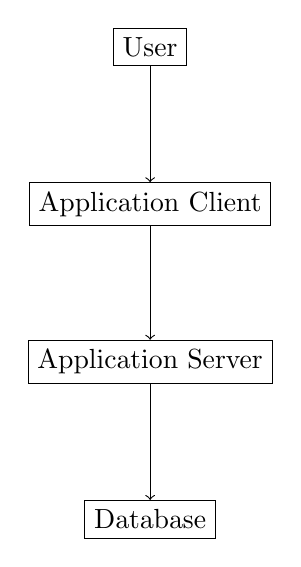
\begin{tikzpicture}[node distance=2cm]
        % Nodes
        \node (user) [rectangle, draw] {User};
        \node (appclient) [rectangle, draw, below of=user] {Application Client};
        \node (appserver) [rectangle, draw, below of=appclient] {Application Server};
        \node (database) [rectangle, draw, below of=appserver] {Database};
        
        % Arrows
        \draw[->] (user) -- (appclient);
        \draw[->] (appclient) -- (appserver);
        \draw[->] (appserver) -- (database);
    \end{tikzpicture}
    \caption{Three-tier Architecture}
\end{figure}



\subsection*{Database Administrator}

A person who has central control over the system is called a database administrator (DBA). The functions of a DBA include:

\begin{itemize}
    \item \textbf{Schema Definition}: Defining the logical structure of the database, including tables, columns, and relationships.
    
    \item \textbf{Storage Structure and Access-Method Definition}: Determining how data is stored on disk and accessed by users and applications.
    
    \item \textbf{Schema and Physical-Organization Modification}: Making changes to the database schema or physical organization to accommodate evolving requirements.
    
    \item \textbf{Granting of Authorization for Data Access}: Managing user permissions and access levels to ensure data security and integrity.
    
    \item \textbf{Routine Maintenance}: Performing regular maintenance tasks to keep the database running smoothly, such as index rebuilds and statistics updates.
    
    \item \textbf{Periodically Backing up the Database}: Creating backups of the database to protect against data loss due to hardware failures, disasters, or human error.
    
    \item \textbf{Ensuring Enough Free Disk Space}: Monitoring disk space usage and ensuring that sufficient space is available for normal operations. Upgrading disk space as required to accommodate growing data volumes.
    
    \item \textbf{Monitoring Jobs Running on the Database}: Monitoring and managing background processes, queries, and other jobs running on the database to ensure optimal performance and resource utilization.
\end{itemize}

By fulfilling these functions, database administrators play a critical role in maintaining the stability, security, and performance of the database system.


\end{document}
